% Setting up the LaTeX document with necessary packages
\documentclass{article}
\usepackage[margin=1in]{geometry}
\usepackage{amsmath,amsfonts}
\usepackage{parskip}
\usepackage{graphicx}
\usepackage{hyperref}
\usepackage{pdflscape} % Added for landscape orientation
\setlength{\parindent}{0pt}

% Beginning the document
\begin{document}

% Defining the title, author, and date
\title{Proposed Architecture for the K-Square Programme Onboarding Agent}
\author{Alberto Espinosa \\ KSquare Group}
\date{1 August 2025}
\maketitle

% Providing an abstract for the document
\begin{abstract}
The K-Square Programme Onboarding Agent streamlines the onboarding of programme execution teams by automating data aggregation and insight generation. This document proposes a robust architecture to support this goal, detailing agentic separation, system layers, and recommended technologies. The architecture leverages LangGraph for agent orchestration, Ollama for local language model inference, and a conversational AI interface with a visual dashboard for user interaction. Four diagrams illustrate the system’s design, providing clarity on agent interactions, data flow, architecture, and high-level workflow.
\end{abstract}

% Introducing the architecture and its purpose
\section{Introduction}
The K-Square Programme Onboarding Agent addresses the challenge of manual onboarding by providing execution teams with rapid access to client profiles, domain knowledge, and actionable insights within 2–3 days. A well-designed architecture is essential to ensure seamless data processing, agent coordination, and user interaction via a conversational interface and visual dashboard. This proposal outlines a layered architecture with six specialised components, focusing on technical feasibility and alignment with enterprise workflows.

% Describing the architecture overview
\section{Architecture Overview}
The architecture is structured into five layers: Data, Agent, Processing, UI, and Orchestration. Six components operate within the system: Programme Setup Agent, Domain Knowledge Agent, Client Profile Agent, Actionable Insights Agent, Meetings Agent, and Knowledge Base. The system integrates internal data from repositories (e.g., SharePoint) and external data from public web sources, delivering outputs through a conversational AI and a visual dashboard. LangGraph orchestrates agent workflows, while Ollama powers local inference for privacy-sensitive tasks.

% Detailing the agentic separation
\section{Agentic Separation}
The system employs five distinct agents and a central Knowledge Base, each with specific roles, inputs, and outputs:

% Describing the Programme Setup Agent
\subsection{Programme Setup Agent}
The Programme Setup Agent guides users through a conversational interface to input project and client details, such as client name, industry, problem statement, and SharePoint links. It queries internal repositories (e.g., SharePoint) and external web sources, validates data sufficiency with users, and routes validated data to the Domain Knowledge and Client Profile Agents. Outputs include structured project profiles stored in the Knowledge Base.

% Describing the Domain Knowledge Agent
\subsection{Domain Knowledge Agent}
The Domain Knowledge Agent aggregates internal and external data to provide domain-specific insights, such as industry best practices and reusable templates. Inputs include validated data from the Programme Setup Agent; outputs include tagged summaries (e.g., definitions, lessons learned) stored in the Knowledge Base, feeding into the Actionable Insights Agent.

% Describing the Client Profile Agent
\subsection{Client Profile Agent}
The Client Profile Agent builds detailed client profiles using internal documents (e.g., statements of work) and public data (e.g., company websites, LinkedIn profiles). It incorporates user validation to ensure relevance, producing tagged profile cards (e.g., stakeholder details, market position) for the Knowledge Base.

% Describing the Actionable Insights Agent
\subsection{Actionable Insights Agent}
The Actionable Insights Agent synthesises outputs from the Domain Knowledge, Client Profile, and Meetings Agents to generate recommendations, summaries, and tasks. Outputs include checklists, one-page summaries, and alerts for pending actions, stored in the Knowledge Base and displayed via the visual dashboard.

% Describing the Meetings Agent
\subsection{Meetings Agent}
The Meetings Agent analyses Microsoft Teams recordings and transcripts to extract action items, scope insights, and engagement metrics. It employs speech-to-text and natural language processing to provide insights that enhance client interactions, storing outputs in the Knowledge Base for the Actionable Insights Agent.

% Describing the Knowledge Base
\subsection{Knowledge Base}
The Knowledge Base centralises tagged data from all agents, including client profiles, domain knowledge, and recommendations. It supports a tagging system for organisation (e.g., Client, Problem Statement, Best Practices) and enables search functionality for internal and external data, feeding the visual dashboard.

% Detailing the system layers
\section{Layer Descriptions}
The architecture comprises five layers, each addressing a critical aspect of the system:

% Describing the Data Layer
\subsection{Data Layer}
The Data Layer manages ingestion, storage, and preprocessing of internal and external data. Internal data (e.g., statements of work, meeting recordings) are retrieved from SharePoint via the Microsoft Graph API. External data (e.g., industry reports, public records) are collected through web crawling. A vector database (e.g., Pinecone) stores document embeddings for semantic search. Preprocessing involves text extraction using optical character recognition (e.g., Tesseract) and chunking with natural language processing libraries (e.g., SpaCy).

% Describing the Agent Layer
\subsection{Agent Layer}
The Agent Layer hosts the Programme Setup, Domain Knowledge, Client Profile, Actionable Insights, and Meetings Agents, coordinated by LangGraph. The Programme Setup Agent initiates data collection via conversational inputs, routing data to other agents. The Knowledge Base stores tagged outputs. Ollama runs local large language models (e.g., LLaMA 3) for internal data processing, with cloud-based models (e.g., OpenAI) for external data.

% Describing the Processing Layer
\subsection{Processing Layer}
The Processing Layer handles language model inference, vector search, and feedback integration. Large language models are fine-tuned using techniques like LoRA for domain-specific accuracy. Vector search, powered by Pinecone or Weaviate, enables rapid document retrieval. A feedback mechanism collects user validations (e.g., relevance scores) to retrain models, targeting 60% initial accuracy with iterative improvement.

% Describing the UI Layer
\subsection{UI Layer}
The UI Layer provides a React-based dashboard with tabs for client profiles, domain knowledge, meeting insights, and recommendations. It features a conversational interface for data input, visual cards for tagged data, and action buttons (e.g., "Generate Checklist"). Chart.js powers visualisations (e.g., engagement metrics), and a REST API (e.g., FastAPI) connects the dashboard to the backend.

% Describing the Orchestration Layer
\subsection{Orchestration Layer}
The Orchestration Layer, powered by LangGraph, manages agent workflows and system monitoring. Workflows are defined as graphs, with nodes representing agent tasks and edges denoting data flow to the Knowledge Base. Monitoring tools (e.g., Prometheus, Grafana) track agent performance and language model accuracy, ensuring reliability and scalability.

% Proposing recommended technologies
\section{Proposed Technologies}
The following technologies are recommended, with justifications and alternatives:

% Describing LangGraph
\subsection{LangGraph}
LangGraph orchestrates agent workflows, enabling dynamic task routing and context retention. It supports complex interactions, such as routing Programme Setup Agent outputs to Domain Knowledge and Client Profile Agents. Its complexity requires experienced developers, but CrewAI is a simpler alternative for prototyping, though less scalable.

% Describing Ollama
\subsection{Ollama}
Ollama enables local language model inference (e.g., LLaMA 3) for processing internal SharePoint documents, ensuring data privacy. Its limitations in large-scale inference necessitate cloud-based models (e.g., OpenAI, Google Gemini) for external data. A hybrid approach balances privacy and performance.

% Listing supporting technologies
\subsection{Supporting Technologies}
\begin{itemize}
    \item \textbf{Pinecone}: A vector database for semantic search, offering scalability. Weaviate is an open-source alternative.
    \item \textbf{Whisper}: OpenAI’s speech-to-text model for transcribing meeting recordings, with high accuracy across languages.
    \item \textbf{FastAPI}: A lightweight framework for building REST APIs to connect the UI and backend.
    \item \textbf{React}: A robust library for an interactive dashboard, styled with Tailwind CSS for responsiveness.
    \item \textbf{Prometheus and Grafana}: Monitoring tools to ensure system reliability and performance.
\end{itemize}

% Presenting the system diagrams
\section{System Diagrams}
The system’s design is illustrated through four diagrams, each presented on a dedicated landscape page for clarity. These diagrams clarify agent interactions, data flow, architectural layers, and the high-level workflow.

% Agents Interaction Diagram
\subsection{Agents Interaction Diagram}
\begin{landscape}
\begin{figure}[p]
    \centering
    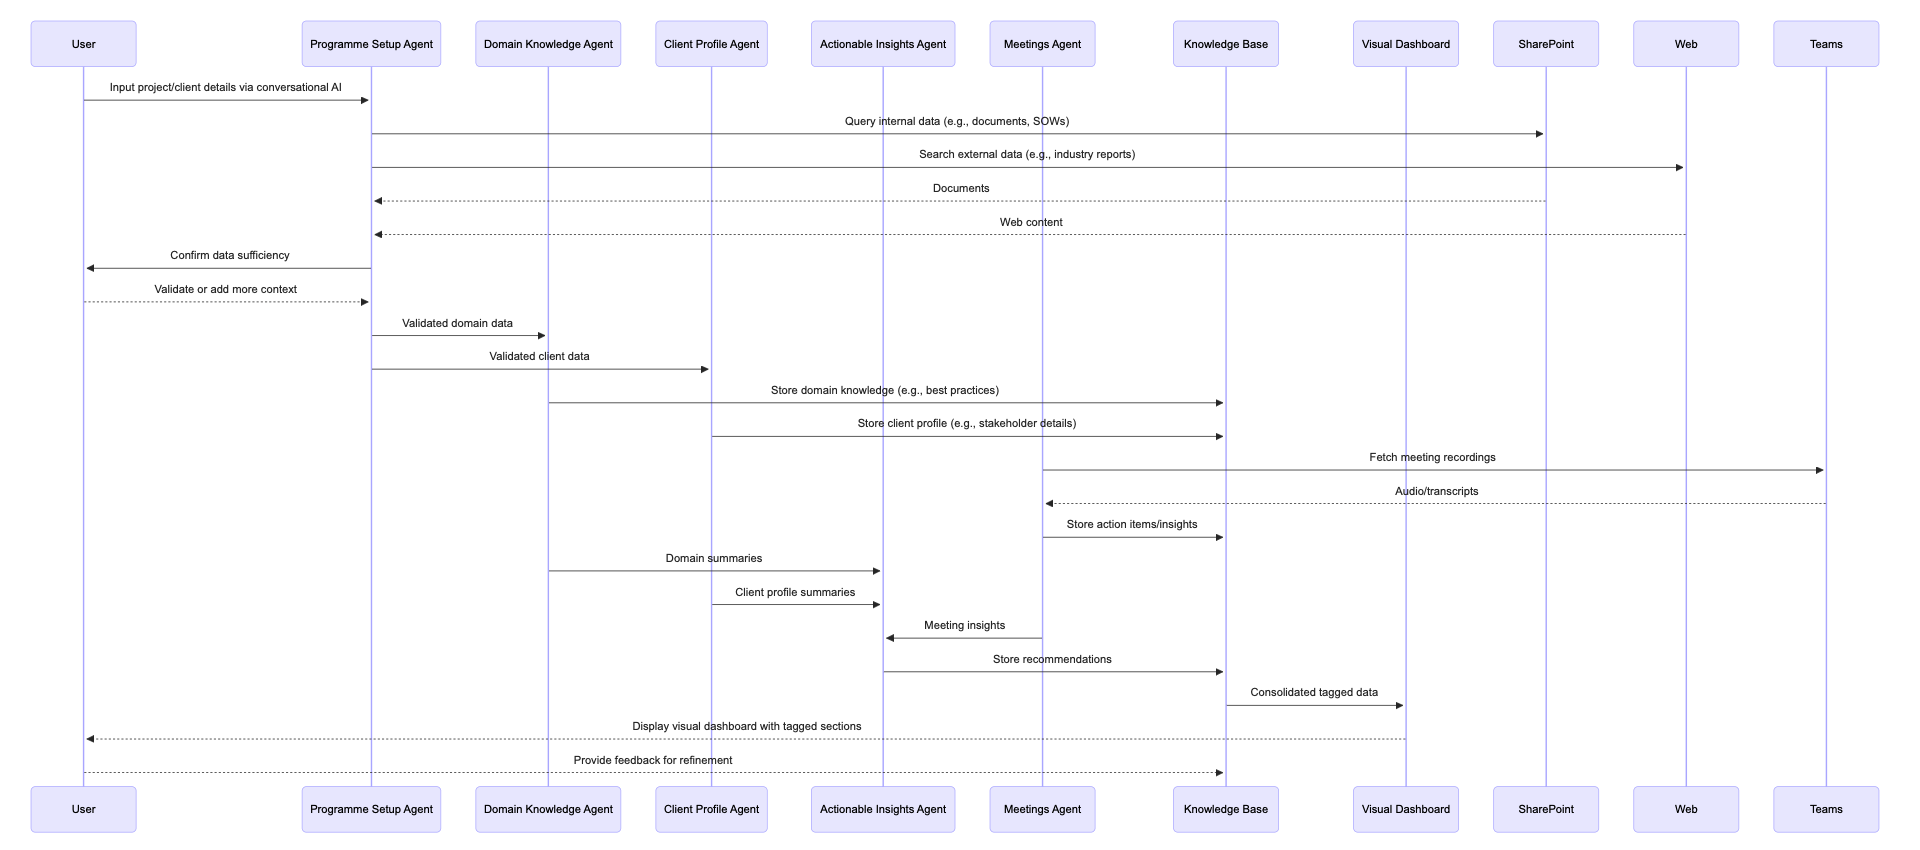
\includegraphics[width=1.5\textwidth]{/Users/albertohernandez/Documents/projects/KS-onboarding/doc/images/agents_interaction.png}
    \caption{Agents Interaction Diagram, showing conversational AI and visual dashboard interactions.}
    \label{fig:agents_interaction}
\end{figure}
\end{landscape}
Figure \ref{fig:agents_interaction} is a sequence diagram illustrating interactions between the User, Programme Setup Agent, Domain Knowledge Agent, Client Profile Agent, Actionable Insights Agent, Meetings Agent, Knowledge Base, and Visual Dashboard. The process begins with users providing project details via a conversational AI, followed by data queries, user validation, and storage in the Knowledge Base. Outputs are displayed in a visual dashboard, with feedback refining agent performance.

% Data Flow Diagram
\subsection{Data Flow Diagram}
\begin{figure}[p]
    \centering
    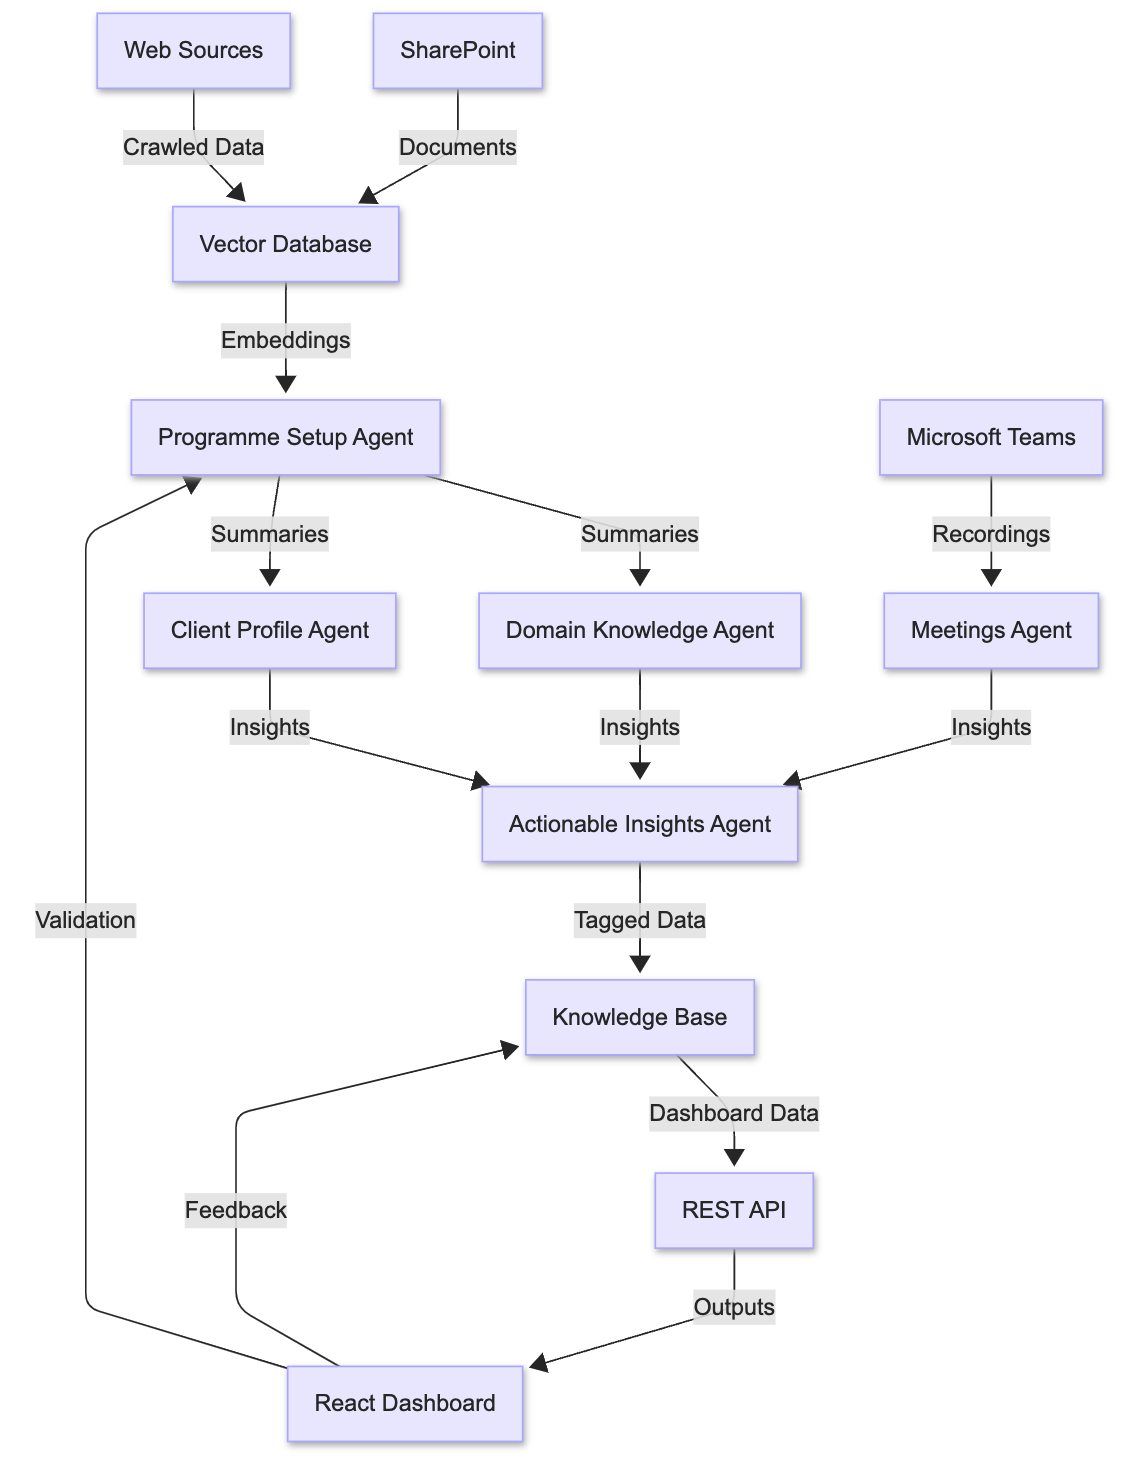
\includegraphics[width=0.8\textwidth]{/Users/albertohernandez/Documents/projects/KS-onboarding/doc/images/data_flow.png}
    \caption{Data Flow Diagram, illustrating data movement through agents and the Knowledge Base.}
    \label{fig:data_flow}
\end{figure}
Figure \ref{fig:data_flow} depicts data flow from SharePoint and web sources to the vector database, Programme Setup Agent, and other agents. Validated outputs are stored in the Knowledge Base, feeding the Actionable Insights Agent and Visual Dashboard via a REST API. Feedback loops refine agent outputs, ensuring a closed-loop system.

% Architecture Diagram
\subsection{Architecture Diagram}
\begin{figure}[p]
    \centering
    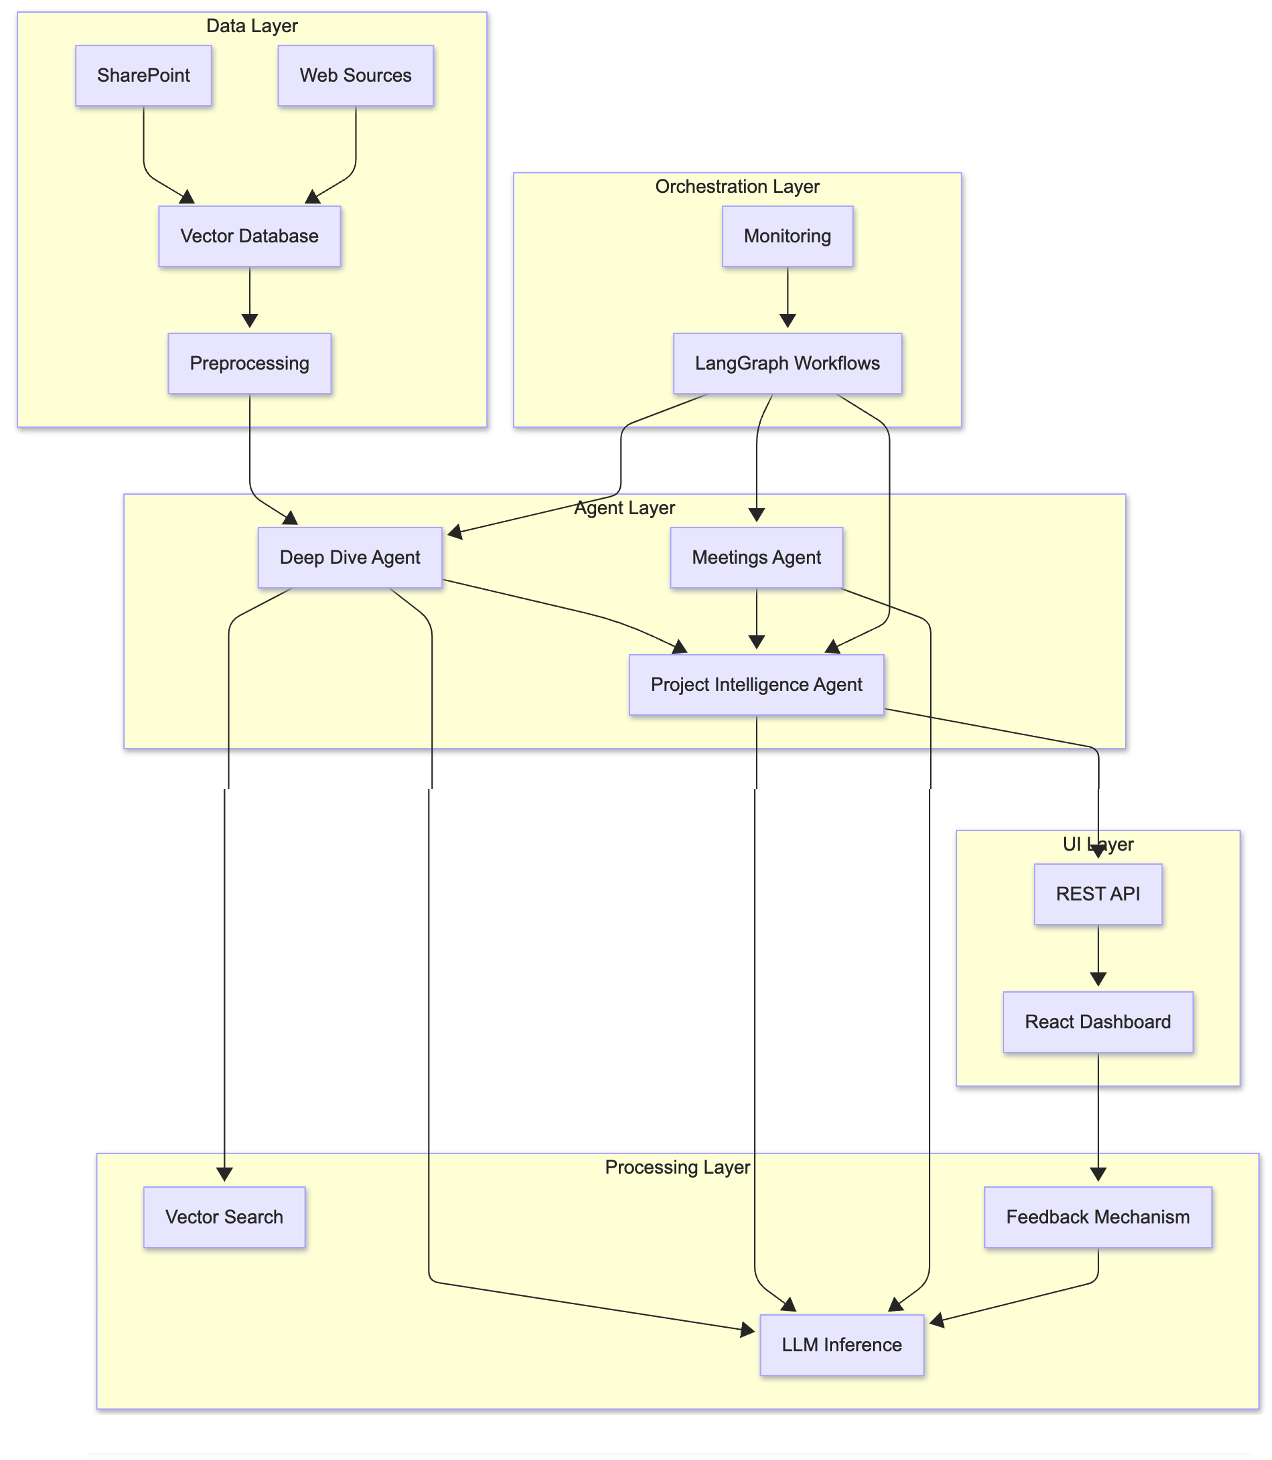
\includegraphics[width=1\textwidth]{/Users/albertohernandez/Documents/projects/KS-onboarding/doc/images/architecture.png}
    \caption{Architecture Diagram, showing the five-layer structure and agent interactions.}
    \label{fig:architecture}
\end{figure}
Figure \ref{fig:architecture} outlines the five layers: Data, Agent, Processing, UI, and Orchestration. The Agent Layer includes the Programme Setup, Domain Knowledge, Client Profile, Actionable Insights, and Meetings Agents, with the Knowledge Base centralising data. LangGraph orchestrates workflows, and the React dashboard delivers outputs via a REST API.

% High-Level Overview Diagram
\subsection{High-Level Overview Diagram}
\begin{figure}[p]
    \centering
    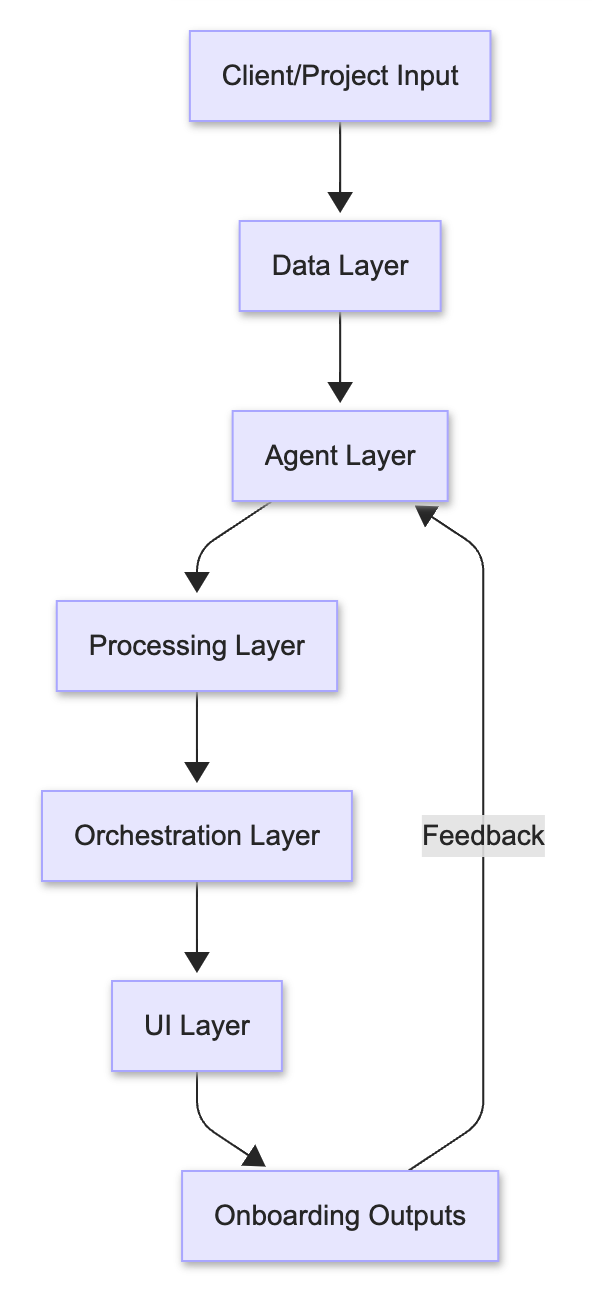
\includegraphics[width=0.5\textwidth]{/Users/albertohernandez/Documents/projects/KS-onboarding/doc/images/overview.png}
    \caption{High-Level Overview Diagram, showing the end-to-end workflow.}
    \label{fig:overview}
\end{figure}
Figure \ref{fig:overview} presents a simplified view of the system’s workflow, from client/project inputs through the Data, Agent, Processing, and Orchestration Layers to onboarding outputs in the UI Layer. Feedback loops ensure continuous improvement.

% Proposing additional features
\section{Suggested Additional Features}
The Meetings Agent utilises speech-to-text and natural language processing to extract insights from meeting data. A novel approach proposed by Espinosa \cite{espinosa2025} introduces a dynamical measurement of opinion change based on semantics and complexity, detailed at \href{https://arxiv.org/abs/2505.02581}{arXiv:2505.02581}. This method uses perturbation and intervention analysis to track conversational dynamics, enabling the Meetings Agent to identify nuanced client perspective shifts. Integrating this feature could enhance insight precision, subject to evaluation for feasibility.

% Concluding the document
\section{Conclusion}
The proposed architecture for the K-Square Programme Onboarding Agent provides a scalable, privacy-conscious solution for automating team onboarding. By leveraging LangGraph, Ollama, and supporting technologies like Pinecone and Whisper, the system ensures robust performance. The conversational AI, visual dashboard, and Knowledge Base enhance usability, while the layered design supports future enhancements, such as advanced conversational analysis.

% Providing the bibliography
\begin{thebibliography}{1}
\bibitem{espinosa2025}
A. Espinosa, ``Embracing Inevitable AI Misalignment as a Strategy to Steer Competitive Agents Towards Human Alignment: Change-of-Opinion Attacks and Interventions,'' arXiv preprint arXiv:2505.02581, 2025.
\end{thebibliography}

% Ending the document
\end{document}